You will use the ultrasonic echo sensor to determine the distance to an object.

\subsection{Theory of Operation}

The ultrasonic echo sensor has a simple interface.
If your program places a logic-high signal on the \lstinline{TRIGGER} pin for 10\textmu s and then drop it to logic-low, then the device will emit a short burst of ultrasound.
The device will then raise the \lstinline{ECHO} pin's logic level to high.
If there is a nearby object, the ultrasound will reflect off of it, and the sensor will detect the echo.
After detecting the echo, the device will drop the \lstinline{ECHO} pin's logic level to low.
If no echo is received, then the device will eventually time-out and drop the \lstinline{ECHO} pin's logic level to low.
After affording the device a quiescent period, the cycle can be repeated.

%Various datasheets\footnote{
%    \url{https://cdn.sparkfun.com/datasheets/Sensors/Proximity/HCSR04.pdf}}$^,$\footnote{\url{https://web.eece.maine.edu/~zhu/book/lab/HC-SR04\%20User\%20Manual.pdf}}$^,$\footnote{\url{https://www.handsontec.com/dataspecs/HC-SR04-Ultrasonic.pdf}
%}\ differ slightly in a few particulars.
%Some describe the time-out period as 36ms, others 38ms.
%Some describe the quiescent period as at least 10ms after the \texttt{Echo} pin's logic drops low; others recommend at least 60ms after the \texttt{Echo} pin's logic goes high.
%The datasheets generally agree that under typical conditions, the device will be able to detect an echo from a $0.5\mathrm{m}^2$ target within 4~meters of the sensor.
%One datasheet suggests that under some conditions, this distance may be as great as 5~meters.\footnote{
%    During testing of the sample solution, sometimes objects 250cm away couldn't always be reliably detected; at other times I was able to detect objects up to 320cm away.
%}

If your program measures the time between the \lstinline{ECHO} pin's logic going high and subsequently going low, then it knows how long the ultrasound travelled to the object and back again.
The classical relationship $distance = speed \times time$ requires that we know how fast the ultrasound travels.

The speed of sound depends on the medium it travels through and the temperature of that medium.
We will assume the medium is air.
\begin{description}
    \item[Old Hardware] If you are using the old hardware, you may assume that the air temperature is 70\degree~Fahrenheit (21.1\degree~Celsius). %21\degree~Celsius (69.8\degree~Fahrenheit).
        The speed of sound for 70\degree\ air is $348.8\frac{m}{s}$.\footnote{
            \url{https://www.weather.gov/epz/wxcalc_speedofsound}
        }
%        The speed of sound for 21\degree\ air is $343.72\frac{m}{s}$.\footnote{
%            \url{https://www.weather.gov/epz/wxcalc_speedofsound}
%        }
    \item[New Hardware] If you are using the new hardware, you will treat the speed of sound as a function air temperature.
        Assuming the temperature $T$ is measured in \degree C, the speed of sound in air is\footnote{
        \url{https://www.weather.gov/media/epz/wxcalc/speedOfSound.pdf}
        }
        \[
%            643.855 \times \sqrt{1 + \frac{T}{273.15}} \times 0.5144444
            331.228 \times \sqrt{1 + \frac{T}{273.15}} \frac{m}{s}
        \]
\end{description}

Thus, by knowing the round-trip travel time, we can determine the distance that the ultrasonic pulse travelled.
The distance to the object it echoed off of will be half of the round-trip distance.

\subsection{The Wrong Calculation}

The internet is littered with example code for measuring distance that instructs you to divide the ultrasonic pulse's round-trip travel time by 58 to obtain the distance in centimeters.
Few of these explain the origin of that particular calculation; however, if you look carefully, you can find one that does.\footnote{
    \url{https://docs.arduino.cc/built-in-examples/sensors/Ping/}
}
Like approximating gravitational acceleration as $10\frac{m}{s^2}$, the calculation of ``divide microseconds by 58'' is simple enough for someone to easily use and provides an adequate approximation.
Like approximating gravitational acceleration as $10\frac{m}{s^2}$, the calculation of ``divide microseconds by 58'' provides you with the wrong answer if ``approximately correct'' is insufficient.

The errors stem from three sources:
\begin{enumerate}
    \item The formulation states that the speed of sound is $340\frac{m}{s}$, but this is the case only when the air temperature is 14.66\degree~Celsius (58.4\degree~Fahrenheit).
        While there are situations in which that \textit{will} be the air temperature, students using the new hardware will measure the temperature, and students using the old hardware will assume the temperature is the thermostat set-point for Avery Hall.
    \item Even if the temperature were 14.66\degree~Celsius, the formulation approximates the speed of sound as $\frac{1}{29}\frac{\mu s}{cm}$, but $\left(340\frac{m}{s}\right)^{-1} = \frac{1}{29.41}\frac{\mu s}{cm}$.
        This rounding error adds up quickly.
    \item On the ATmega328P microcontroller (which most of the examples are targeting), the timer typically used to measure time is only accurate to within 4\textmu s.
        Even if $\frac{1}{29}\frac{\mu s}{cm}$ were the correct expression, this will produce an error of about 1mm.
        If we were using floating point arithmetic, this could be dismissed as a rounding error, but we are using integer arithmetic.
        Because integer division truncates the fractional portion of the quotient, there will be times in which ``round-towards-zero'' produces an error of a full centimeter relative to the answer that a more-careful computation would have produced.
\end{enumerate}


\subsection{The Correct Calculation}

\subsubsection{Practical Considerations}

\paragraph{Arithmetic}

As neither of our microcontrollers have a floating point unit (FPU), we want to avoid floating point calculations, which are computationally expensive when performed entirely in software.
Further, the ATmega328P cannot perform division in hardware, and so we want to avoid integer division unless the divisor is a power of two when using the old hardware.
The RP2040 has an integer divider that requires 8 processor clock cycles to perform division, so we might allow integer division with the new hardware -- but we have an equation that will not require the integer divider.

\paragraph{Time}

After we configure a timer to manage the sensor, we will be able to use its counter to determine the round-trip travel time.
On the old hardware, the ``tick'' will be a half-microsecond.
On the new hardware, the ``tick'' will be one microsecond.

\subsubsection{The Equations}\label{subsubsec:equations}

These equations can be used to accurately compute the distance to an object.
That is, the computed distance is half of the ultrasonic pulse's round-trip distance.
The derivation of these equations can be found in Appendix~\ref{sec:distanceFormulation}.

\paragraph{Old Hardware}

\[
    distance = time_{\mathrm{half}\mu s} \times \frac{18,025 cm}{\mathrm{half}\mu s} \div 2^{21}
\]

Even though $distance$ will be less than 500~cm, you will need at least 31 bits to represent the intermediate products when performing the arithmetic.

\paragraph{New Hardware}

\[
    distance = time_{\mu s} \times \left( 256,108,888 - 121,907 \times ADC\_register\_value \right) \frac{cm}{\mu s} \div 2^{33}
\]

Even though $distance$ will be less than 500~cm, you will need at least 44 bits to represent the intermediate products when performing the arithmetic.

\textcolor{red}{Obtaining the $ADC\_register\_value$ will be treated as extra credit.
If you do not wish to pursue that extra credit, then you may hard-code $ADC\_register\_value$ as 889, which is the value corresponding to 21.05\degree C (69.9\degree F).}

%There is also a practical consideration with respect to the sensor itself.
%Sound isn't particularly directional.
%The horns surrounding the ultrasonic transducers help to limit the ``beam width,'' but only to a degree.
%Pointing the sensor straight down an otherwise empty hallway, you will probably still detect a reflection from the walls to either side.\footnote{
%    If you're feeling nerdy, you could use right-angle trigonometry to determine the ``beam width'' --
%    point the sensor straight at a wall to determine how far away from it you are (the ``opposite''), then point the sensor parallel to the wall and take a reading (the hypoteneuse).
%    Divide the ``opposite'' by the hypoteneuse and take the arcsin -- the resulting value is the angle from straigth-ahead to how far to the right/left the sensor will detect a reflection.
%}



\subsection{Examining the Starter Code}

The \function{initialize_sensor()} function is where you'll place any alarm-related code that needs to be run once when the program starts.
The \function{manage_sensor()} function is where you'll place any alarm-related code that needs to run with every iteration of the program's main loop.
You will, of course, add code outside these functions too: an interrupt service routine for a timer, an interrupt handler for the distance sensor, and possibly helper functions.

\subsection{Single-Pulse Operation} \label{subsec:distanceSinglePulseOperation}

\begin{description}
    \checkoffitem{Create a variables to:
        \begin{itemize}
            \item indicate whether an object has been detected
            \item indicate the object's distance (if the object is detected)
            \item indicate the object's rate of approach (this will only be useful in Normal Operation mode)
        \end{itemize}
        Be sure to declare them not only in \textit{sensor.c} (without the \lstinline{extern} modifier) but also in \textit{shared\_variables.h} (with the \lstinline{extern} modifier).
    }
    \checkoffitem{In \function{initialize_sensor()}, initialize the object detection variable to indicate that an object has not been detected.}
\end{description}

A fully-correct implementation of Single-Pulse Operation mode has the alarm chirp if an object is detected closer than the threshold range (Requirement~\ref{spec:singlePulseOperation}).
For now, your focus will be on determining the distance to an object.

\begin{description}
    \checkoffitem{In \textit{sensor.c}, create a temporarily-empty interrupt handler that will be used to respond to the sensor timer's interrupts.
        Don't forget to pre-declare this functions above \function{initialize_sensor()}.}
    \checkoffitem{In \function{initialize_sensor()}, register that function as an ISR for a timer interrupt that has a period of 32,768\textmu s}
        \begin{itemize}
            \item On the old hardware, use TIMER1.
            \item On the old hardware, this should configure TIMER1 to have a ``tick'' of $\frac{1}{2}\mu s$ (which we will refer to as $1\mathrm{half}\mu s$).
                On the new hardware, the timer's ``tick'' will be $1\mu s$
        \end{itemize}
\end{description}

%Using the ``Timers'' section of the Cow Pi datasheet,\footnote{
%    \url{https://cow-pi.readthedocs.io/en/latest/microcontroller.html\#timers}
%}
%place code in \function{initialize_sensor()} to configure Timer1 to produce an \textbf{overflow} interrupt every 32,768\textmu s, using the ``Normal'' mode.
%Place in \function{initialize_sensor()} code to enable that interrupt.

\begin{description}
    \checkoffitem{Create a state machine for the sensor that can be ``initial-start'', ``powering-up'', ``ready,'' ``active-listening,'' ``active-detected,'' and ``quiescent.''}
    \checkoffitem{Initialize that state machine to be ``initial-start''.}
\end{description}

\textit{If you are using the new hardware}, you will need to be able to read from an analog-digital converter (ADC).
\begin{description}
    \checkoffitem{Create a pointer to an \lstinline{adc_t} structure and point it to \lstinline{0x4004c000}.}
    \checkoffitem{In \function{initialize_sensor()}, configure the ADC using its \lstinline{control} register:}
        \begin{itemize}
            \item Set bit20 to \lstinline{1} indicating that we are interested in ADC channel 4.
            \item Set bits14..12 to \lstinline{4} indicating that channel 4 is the next channel to convert.
            \item Set bits1..0 to \lstinline{3} indicating that the temperature sensor should be powered, and that the ADC should be enabled.
        \end{itemize}
\end{description}


\begin{figure}[h]
    \centering
%    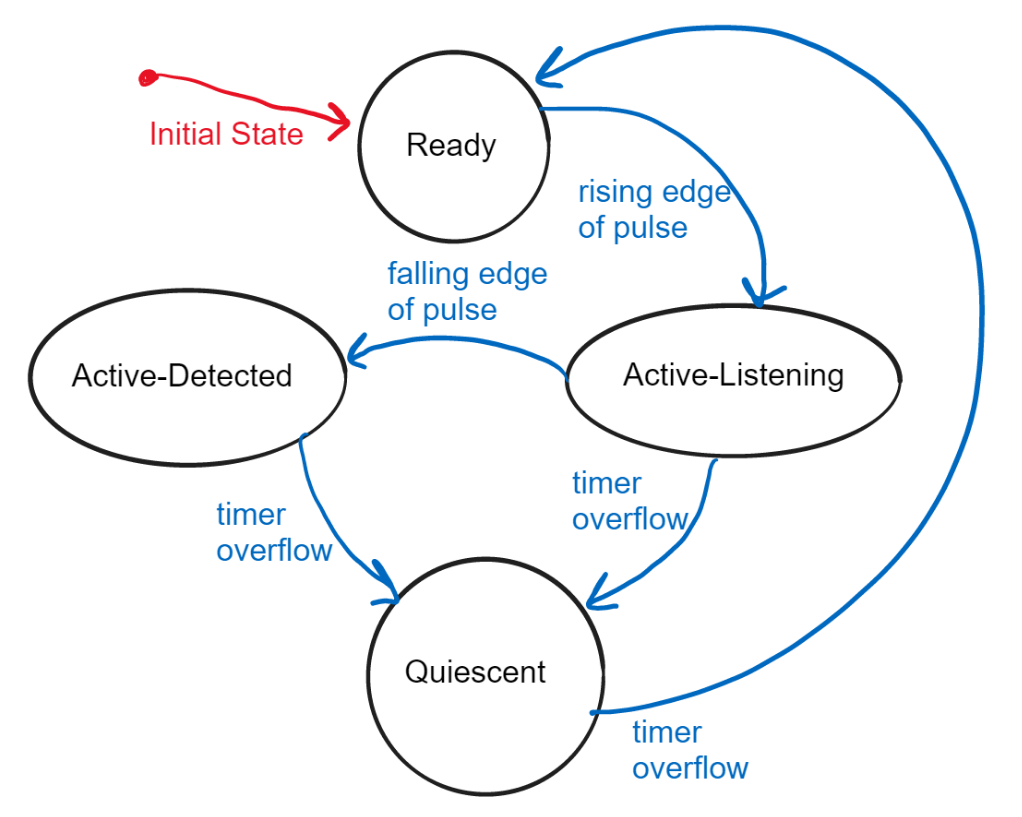
\includegraphics[width=3in]{sensorStateMachine}
    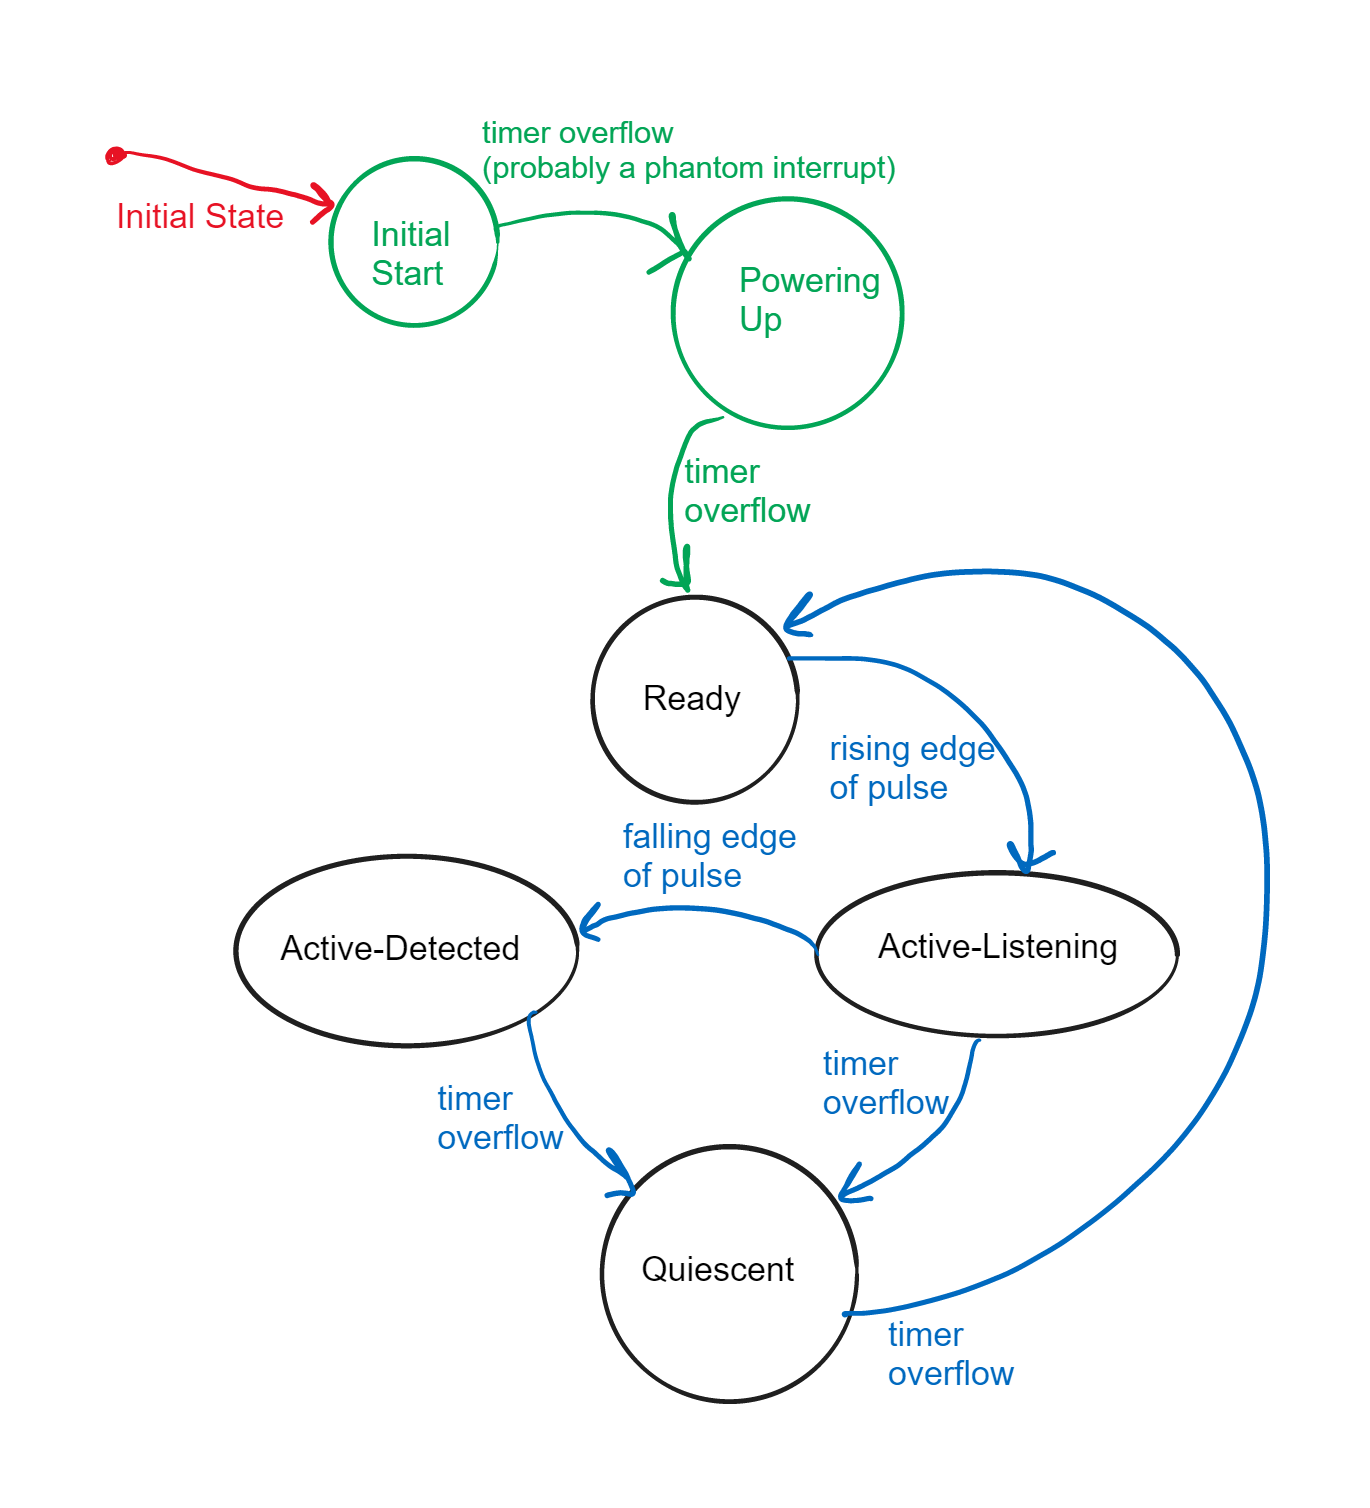
\includegraphics[width=4in]{noPhantomInterrupts}
    \caption{\label{fig:sensorStateMachine} State machine describing the control of the distance sensor.
%        See Appendix~\ref{sec:phantom} for an alternative state machine.
    }
\end{figure}

%Use the \function{ISR} macro to create an interrupt service routine in \textit{sensor.c} for that interrupt.
%Leave the ISR's body empty for now.

\begin{description}
    \checkoffitem{In \textit{sensor.c}, create a temporarily-empty interrupt handler that will be used to detect the rising and falling edge of the pulse. %one for actions to be taken when the sensor emits its ultrasound pulse, and one for actions to be taken when the sensor receives an echo.
        Don't forget to pre-declare this functions above \function{initialize_sensor()}.}
        \begin{itemize}
            \item \textcolor{red}{\textbf{Do \textit{NOT} use \function{manage_sensor()} as your interrupt handler!}}
        \end{itemize}
    \checkoffitem{Place in \function{initialize_sensor()} code to register the handler for a CHANGE on the \lstinline{ECHO} pin.}
\end{description}

\paragraph{Allow Time for the System to Initialize}

When the system starts up, the input pins and the timers may fire ``phantom'' interrupts.
We will handle this taking no action until the sensor timer has fired at least two interrupts.

In the timer interrupt handler:
\begin{description}
    \checkoffitem{If the sensor's state machine is in its ``initial-start'' state, place it in its ``powering-up'' state}
    \checkoffitem{If the sensor's state machine is in its ``powering-up'' state, place it in its ``ready'' state}
\end{description}

\paragraph{Initiate a Pulse}
Place code in \function{manage_sensor()} that, whenever a ping is requested (see Section~\ref{subsec:readPushbutton}), will:
\begin{description}
    \checkoffitem{First, set the \lstinline{TRIGGER} pin to logic-high}
    \checkoffitem{Then, set the variable indicating that a ping is requested to \lstinline{false}}
    \checkoffitem{Next, delay for 10\textmu s}
    \begin{description}
        \item[Old Hardware] \phantom{x} \\
        \begin{itemize}
            \item You will need a pointer to TIMER1
            \item Use the timer's counter to busy-wait for 20half\textmu s
        \end{itemize}
        \item[New Hardware] \phantom{x} \\
        \begin{itemize}
            \item You will need a pointer to the general-purpose timer
            \item Use the timer's counter to busy-wait for 10\textmu s
        \end{itemize}
    \end{description}
    \checkoffitem{Finally, set the \lstinline{TRIGGER} pin to logic-low}
\end{description}

Several microseconds later, the sensor will emit its ultrasound pulse and raise its \texttt{Echo} line to logic-high.

\paragraph{Handle the Start of a Pulse}
In the function that you registered to handle the pulse edges on the \lstinline{ECHO} pin, you want to keep track of whether the interrupt handler was triggered for a rising or falling edge.
While you \textit{could} do so by checking the logic level on the \lstinline{ECHO} pin, you can also assume that rising and falling edges alternate --
you will never have two rising edges in a row, and you will never have two falling edges in a row.

If the pin interrupt handler was triggered for a rising edge, you want to start the process of determining exactly how much time passes between emitting the pulse and receiving the echo.
\begin{description}
    \checkoffitem{First, reset the sensor timer's}
    \checkoffitem{Then, \textit{if you are using the new hardware}, copy the value of the timer's counter into a \lstinline{volatile} global variable}
        \begin{itemize}
            \item You will need a pointer to the general-purpose timer
            \item \textit{For the old hardware}, the timer's counter will be 0 after resetting the timer, so copying it is not necessary.
        \end{itemize}
    \checkoffitem{Finally, place the sensor state machine in its ``active-listening'' state}
\end{description}

Two things will happen in the next 38 (or fewer) milliseconds: the signal on the \lstinline{ECHO} pin will fall to logic-low, and the sensor timer will fire an interrupt.
Whichever happens first, the signal falling low or the timer interrupt, will tell us whether there's an object.

\paragraph{Handle the End of a Pulse}
If the signal on the \lstinline{ECHO} pin falls to logic-low first, then it's because there's an object that reflected the ultrasound pulse.

If the pin interrupt handler was triggered for a falling edge, and if the sensor is ``active-listening,'' then you want to capture the information needed to compute the distance.
\begin{description}
    \checkoffitem{First, copy the value of the timer's counter into a \lstinline{volatile} global variable}
        \begin{description}
            \item[Old Hardware] \phantom{x} \\
                \begin{itemize}
                    \item You will need a pointer to TIMER1
                    \item The value that you copy is the number of half-microseconds between the pulse emission and the echo's return
                \end{itemize}
            \item[New Hardware] \phantom{x} \\
                \begin{itemize}
                    \item You will need a pointer to the general-purpose timer
                    \item This value, minus the value you copied at the start of the pulse, is the number of microseconds between the pulse emission and the echo's return
                \end{itemize}
        \end{description}
    \checkoffitem{Then, place the sensor state machine in its ``active-detected'' state}
\end{description}

\paragraph{Handle Timer Interrupt}

If the sensor timer overflows before the signal on the \lstinline{ECHO} pin falls low, then there is not an object within detectable range.
The sensor will time-out after 36,000--38,000\textmu s, and the sensor timer will fire an interrupt after 32,768\textmu s.
Any object whose echo might have been detected after this must be beyond the sensor's detection range.

If the sensor is ``active-listening'' then no object was detected:
\begin{description}
    \checkoffitem{First, indicate that an object has not been detected}
    \checkoffitem{Then, place the sensor in its ``quiescent'' state}
\end{description}

On the other hand, if the sensor is ``active-detected'' then an object was detected:
\begin{description}
    \checkoffitem{First, indicate that an object has been detected}
    \checkoffitem{Then, place the sensor in its ``quiescent'' state}
\end{description}

As noted above, the sensor requires quiescent period between pulses.
We shall allow 65.536ms between pulses, which is ample time for a quiescent period.

If the sensor is ``quiescent'' when the timer interrupt fires:
\begin{description}
    \checkoffitem{Place the sensor in its ``ready'' state}
\end{description}


\paragraph{Compute and Display the Distance}

Add code to the \function{manage_sensor()} function that, if an object has been detected, computes the distance (as a whole number of centimeters) to the object.
\begin{description}
    \item[Old Hardware] If an object has been detected, then from handling the end of the pulse, you have the number of half-microseconds that the pulse was high.
        \begin{description}
            \checkoffitem{Use the equation from Section~\ref{subsubsec:equations} to compute the distance.}
                \begin{itemize}
                    \item \textcolor{red}{Do not use \function{pow()} to compute $2^{21}$} -- remember, we're trying to avoid floating point calculations
                    \item If you think back to chapter~3, you'll realize that you do not need to compute $2^{21}$
                \end{itemize}
        \end{description}
    \item[New Hardware] If an object has been detected, then you have the time that the pulse initiated (from handling the start of the pulse) and the time that the pulse ended (from handling the end of the pulse).
        \begin{description}
            \checkoffitem{Compute the length of time that the pulse was high.}
            \item[If you are not pursuing the temperature extra credit] \phantom{ }
                \begin{description}
                    \item Hard-code $ADC\_register\_value$ as 889
                \end{description}
            \item[If you are pursuing the temperature extra credit] Read the ADC channel that the temperature sensor is connected to.
                Using your \lstinline{adc_t} pointer:
                \begin{description}
                    \checkoffitem{Set \lstinline{control} register's bits14..12 to \lstinline{4} indicating that channel 4 is the next channel to convert.}
                    \checkoffitem{Set the \lstinline{control} register's bit2 to 1, indicating that we want a conversion.}
                        \begin{itemize}
                            \item The ADC will automatically set \lstinline{control}'s bit8 to become 0, indicating that a conversion is in progress.
                        \end{itemize}
                    \checkoffitem{Busy-wait while \lstinline{control}'s bit8 is 0}
                    \begin{itemize}
                        \item When the ADC automatically sets \lstinline{control}'s bit8 to 1, it indicates that it is ready for the next conversion.
                    \end{itemize}
                    \checkoffitem{Copy the ADC result from the \lstinline{result} register.}
                \end{description}
            \checkoffitem{Use the equation from Section~\ref{subsubsec:equations} to compute the distance.}
            \begin{itemize}
                \item \textcolor{red}{Do not use \function{pow()} to compute $2^{33}$} -- remember, we're trying to avoid floating point calculations
                \item If you think back to chapter~3, you'll realize that you do not need to compute $2^{33}$
            \end{itemize}
        \end{description}
    \checkoffitem{Display the clearly-labeled distance on the display module.}
    \checkoffitem{Now add code to the \function{manage_sensor()} function that, if an object has \textit{not} been detected, displays on the display module a clear indication that there is no detected object.}
\end{description}
As a small optimization, you might have your code make these updates only when the sensor is ``quiescent.''

\vspace{0.5cm}

Test your code.
I recommend that you place your Cow~Pi on top of its food-container carrying case, or some other object, to reduce the likelihood of the sensor receiving an echo from your worktable.

\vspace{0.5cm}

Most of the work to configure the alarm for Single-Pulse Operation takes place in Section~\ref{subsec:soundSinglePulseOperation}.
You will finish implementing Single-Pulse Operation in Section~\ref{subsec:integrationSpeedSinglePulseOperation} by integrating the detection code from Section~\ref{subsec:distanceSinglePulseOperation} with the alarm code from Section~\ref{subsec:soundSinglePulseOperation}.
This will require small changes to the code.
